\chapter{The RITAS algorithm}
\label{sec:ritas}

Our algorithm constructs yield maps through the following steps:
Rectangle creation, Intersection assignment, Tessellation,
Apportioning, and Smoothing (RITAS). The overarching goal of this
process is to mimic the real world harvesting processes. Figure
\ref{fig:closeup} provides an illustration of a subset of these steps.

\begin{figure}[h!]  \centering
  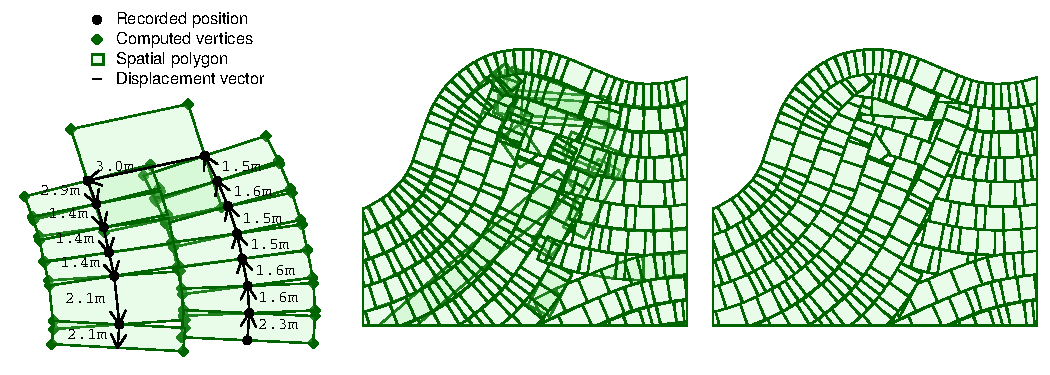
\includegraphics[width=\textwidth]{algoplots}
  \caption[Close-up illustration of selected algorithm steps]{Close-up
    illustration of selected processing steps. \underline{Left}:
    Construction of the vehicle polygons from the GPS location
    data. Black dots mark the location at the end of each logging
    cycle, green dots correspond to the vertices computed according to
    the displacement vector implied by two consecutive spatial
    points. The distance traveled could be reported by the yield
    monitor or estimated from the vector length. \underline{Center}:
    Spatial polygons reveal overlap (darker areas) due to driving
    maneuvers. \underline{Right}: Tessellation eliminates the overlap
    by assigning intersecting areas to the first polygon in time.}
    \label{fig:closeup}
\end{figure}

Each precision yield data set is assumed to have time-ordered rows
containing the following information: mass harvested $m_t$,
2-dimensional spatial coordinate $(x_t,y_t)$, and swath half-width
$w_t$ for $t=0,\ldots,T, \ T \in \mathbb{N}$.  We assume any lag time
has been effectively pre-processed by appropriately matching the mass
harvested to its 2-dimensional location. See, for example,
\cite{Burks2004, Hemming2005, Sudduth2007, Sudduth2012}.

\paragraph*{Step 1: Rectangle creation}

Figure \ref{fig:closeup} (left) illustrates the construction of a
rectangular polygon representing the harvested area between each
sequential pair of spatial coordinates. The position vector
$\mathbf{s_t} = (x_{t}, y_{t})$ represents the location of the tracked
device in a 2-dimensional plane at the time step $t$, which we assume
to be the midpoint of the combine harvester head. The rectangle is
then uniquely identified by the position of its four vertices, two
representing the beginning of the harvested area at time step $t-1$
and two representing the end of the harvested area at time step
$t$. The linear displacement vector is equal to the vector difference
between the position vectors at two subsequent time steps
$\mathbf{s_t} - \mathbf{s_{t-1}}$. The first two vertices are computed
as the endpoints of a line segment perpendicular to the displacement
vector with midpoint at $\mathbf{s_{t-1}}$ and length equal to the
swath width $2 w_t$. The remaining two vertices are found using the
same procedure but pivoting on the midpoint $\mathbf{s_t}$
instead. Given a pair of position vectors
$\mathbf{s_t}, \mathbf{s_{t-1}}$, denote
$b_t = (y_t - y_{t-1}) / (x_t - x_{t-1})$ the slope of the connecting
line, and define $dx_t = w_t (1 + b_t^{-2})^{-\frac{1}{2}}$ and
$dy_t = - dx_t b_t^{-1}$. Then, the rectangle associated with mass
$m_t$ has the four vertices coordinates given by
$\{(x_{i} \pm dx_t, y_{i} \pm dy_t): i = t, t-1\}$.

As the first spatial point has no displacement, this processing yields
$T$ rectangles with vertices collected in the set
$\mathcal{P} = \{P_{\tau}$: $\tau \in \{1, \dots, T\}\}$.

\paragraph{Step 2: Intersection assignment and Tessellation}

\OUTLINE{Motivate clipping} Figure \ref{fig:closeup} (middle) shows
end result of this construction which produces rectangles that
overlap, an area called the \emph{intersection}, due to adjacent
harvester paths. Geometries in $\mathcal{P}$ represent the area over
which the combine harvester passed, which may differ from the
effectively harvested area at each time step since the header may not
be full of crop when harvesting the field boundaries (e.g. on outer
edges, around voids), or within them. As a byproduct of the
destructive sampling scheme, the discrepancy is linked to the spatial
superposition of the observational units that arise due to local
harvesting dynamics such as turns, wedges, parallel lines, and
traveling over harvested areas. Globally within a field, this
phenomenon can be exacerbated by factors such as field
characteristics, or narrow row crops \cite{Ross2008}. Generally,
overlapping cannot be assumed symmetrical nor time-invariant. For
example, pivoting motions overlap on the inner side and the proportion
of duplicated area varies at each time step depending on factors such
as the sharpness of the turns, the angle of the wedges, or the
obstacles faced by the operator.

\OUTLINE{Explain clipping} As a general framework to model the
time-varying effectively harvested area, we run a time-ordered
apportioning procedure over the rectangles in $\mathcal{P}$. Let
$\tilde{P}_\tau = P_t \setminus \left( \bigcup_{i = 1}^{t - 1} P_i
\right)$ be the time-ordered relative complement of the previously
harvested area in the rectangle corresponding to the time step $t$. By
doing this, we effectively map the set of overlapping rectangles
$\mathcal{P}$ into a set of non-overlapping polygons
$\tilde{\mathcal{P}} = \{\tilde{P}_{\tau}: \tau \in \{1, \dots, T
\}\}$. When the original dataset has no voids (e.g. unplanted,
flooded, or more generally inaccessible sub areas),
$\tilde{\mathcal{P}}$ form a flat plane covered by tiles with no
overlaps and no gaps (non-periodic tessellation). Some of the
computational considerations discussed in \cite{Drummond1999}, such as
the time scaling and appropriate techniques to reduce algorithm
complexity, are relevant for implementing this step.

This step creates $T$ polygons partitioning the harvested area, each
associated with the same mass it had in Step 1 but now the area may be
smaller (due to the intersection removal) and thus yield is more
accurately captured.

\paragraph*{Step 3: Apportioning} \OUTLINE{Motivate
  gridding \& apportioning} The elements in $\tilde{\mathcal{P}}$ are
unsuitable for spatial techniques that do not accommodate areas with
irregular shapes and heterogeneous area sizes. Two equally-sized long
rectangles, one in a vertical and the other in a horizontal position,
would have the same centroid yet they convey different information
about yield to the north or west of the centroids. Alternatively, two
centered equally-shaped polygons with different sizes carry different
information about the spatial coverage of the collected
data.

To normalize the areal representation in terms of both shape and size,
we superimpose a regular grid of square pixels, assign portions of the
polygons into grid pixels, and apportion the harvested mass associated
with the polygons to the pixels. The first two steps involve topology
operations on geometries whereas the last one involves manipulation of
the numerical data. Accounting for these two spatial features is by
itself a methodological improvement over the surveyed algorithms,
which simply reduce data to spatial points such as the displacement
vector endpoint or, less commonly, the polygon centroid.

\OUTLINE{Explain gridding \& apportioning} Let $\mathcal{P}^{*}$ be
a set of $N \in \mathbb{N}$ equally-sized, non-overlapping, and
contiguous squared pixels forming a partition covering all the
elements in $\tilde{\mathcal{P}}$. The constant $N$ reflects the user
preference in terms of resolution, selected either by the total number
of pixels, more intuitively by the pixel length in meters, or the
target computational time investment. Although pixels size can be set
arbitrarily, its choice should consider the accuracy of the position
system. We take the pairwise intersection among the elements in
$\tilde{\mathcal{P}}$ and $\mathcal{P}^{*}$ and compute
$\pi_{\tau, n} \in [0, 1]$ the proportion of the area in the $\tau$-th
non-overlapping polygon $\tilde{P}_{\tau}$ that intersects with the
$n$-th pixel in the grid for $\tau \in \{1, \dots, T\}$ and
$n \in \{1, \dots, N\}$. The corresponding proportion of the harvested
mass $m_{\tau}$ associated with $\tilde{P}_{\tau}$ is assigned to
$P^{*}_n$. The total harvested mass associated with the $n$-th pixel
is given by $m^{*}_n = \sum_{\tau = 1}^{T} \pi_{\tau, n} \
m_{\tau}$. The resulting polygons in $\mathcal{P}^{*}$ resemble much
the Basic Areal Units (BAUs) as defined by \cite{Nguyen2012} in the
context of massive data fusion: fine-scale, nonoverlapping, areal
regions representing the smallest resolution at which data is
aggregated.

\OUTLINE{Apportioning key fact (1)} Two key aspects behind the
gridding strategy are worth mentioning. First, for the purpose of
apportioning, we assume that the harvested mass associated with the
spatial polygons is distributed uniformly within each unit. This is a
sensible assumption in this context as combine harvester log data in
short cycles and the spatial polygons represent small areas for the
scale of the underlying crop growth process.

\OUTLINE{Apportioning key fact (2)} Second, if one imposes regularity
and equal-shape conditions on the grid elements and also forces it to
cover all the elements in $\tilde{\mathcal{P}}$, the sum of the
pixels area may exceed the sum of the tessellated polygons area. The
excess, found at both the harvested region outer borders and the inner
voids boundaries, can be diagnosed visually with ease. It decreases as
the grid resolution, or equivalently as the total number of pixels
$N$, increases and so can be controlled at the cost of additional
computational time for topology operations and smoothing. %More
Concretely, when a Gaussian Process is applied for smoothing as
described below, exact inference has time complexity in the order of
$O(N^3)$ and storage demands of of $O(N^2)$. In other words, as we
double the map resolution, we octuple the number of operations and
quadruple the need for storage.  Alternatively, one could exclude the
pixels with less than an arbitrary proportion of area effectively
covered by the tessellated observations. A sensible choice, such as a
minimum coverage of 50\%, will tend to balance under and over-covered
polygons. Due care should be taken so that apportioning is still
applied validly: mass should be allocated to pixels only in proportion
of the actual overlapping area, discarding any part of the tessellated
polygons that is not covered by any pixel. Note that the grid
resolution serves only for the purpose of spatial aggregation, and
need not be the same resolution used for the visualization that will
be introduced in the following step.

This step creates $N$ polygons, determined by the user based on
tesselation resolution, partitioning the harvested area each with an
associated mass of harvested crop. Figure
\ref{fig:basswood2012-main-steps} (bottom left) shows the regular grid
with apportioned mass. The regular tesselation provides constant areas
and meaningful centroids, and therefore we can use standard spatial
smoothing techniques directly on mass, as opposed to yield.

\paragraph{Step 4: Smoothing} \cite{McCullagh2006} provided empirical
evidence suggesting that the non-anthropogenic spatial variation in
yield, defined as patterns that cannot be explained by topography or
human intervention, matches the characteristics of the de Wijs process
plus white noise. We smooth using a Gaussian Process (GP) with a
Mat\'ern covariance on the logarithm of mass
\citep{handcock1993bayesian,gutt2006studies}, which becomes similar to
a de Wijs process as the length scale tends to zero. Compared with the
more common powered exponential covariance functions, e.g. Gaussian or
exponential, the Mat\'ern adds an additional parameter that controls
local smoothness, i.e. \ differentiability, and therefore is often
more accurate for real world processes.

Covariance parameters are estimated via Maximum Likelihood, and
smoothed values are found for each tile following \cite{Cressie1993}.
Specifically, for each pixel we have a predicted mean
$\hat\mu_{\ell} \in \mathbb{R}$ and variance
$\hat\sigma^2_{\ell} > 0$ for the logarithm of mass.  We using the
following formulas to convert back to the mean and variance of mass
\[ \hat{\mu}_{m} = \exp\left(\hat{\mu}_{\ell} +
\hat{\sigma}^2_{\ell}/2\right), \quad\mbox{and}\quad
\hat{\sigma}^2_{m} = \exp\left(2 \hat{\mu}_{\ell} +
\hat{\sigma}^2_{\ell}\right)
\left[\exp\left(\hat{\sigma}^2_{\ell}\right) - 1\right].
 \] Finally, yield is calculated by dividing the tile mass by the tile
area.

We have implemented our algorithm in the R programming language, using
the R packages doParallel, foreach, gstat, rgeos, and sp
\citep{Pebesma2004, Pebesma2005, Bivand2013, Graeler2016,
  Microsoft2017, Corporation2018, RCT2019, Bivand2019}.
% Our open-source
% `yieldMaps` package contains routines for the algorithm described in
% the article, visualization routines, and the dataset employed in the
% case study. The algorithm routines were programmed as smaller, modular
% tasks so that users could easily adapt the source code to custom needs
% such as designing a different gridding and aggregation strategy, or
% employing another spatial interpolation model. Visualization routines
% include map generation as well as object movement and polygon creation
% visualizations.

%%% Local Variables:
%%% mode: latex
%%% TeX-master: "../thesis"
%%% End:
